\documentclass[10pt, aspectratio=169]{beamer}

\usepackage[T1]{fontenc}
\usepackage[utf8]{inputenc}
\usepackage[slovene]{babel}
\usepackage{lmodern}
\usepackage{amsfonts,amssymb,amsmath}
\usepackage{pgfpages}
% \usepackage{tikz}
\usepackage{wrapfig}
\usepackage{graphicx}
\usepackage{pgfkeys}
\usepackage{pgfplots}
\usepackage{xcolor}
\usepackage{tkz-euclide}
\usepackage{xfp}
% \usepackage{pgf}

\usetikzlibrary{angles,arrows,arrows.meta,calc,decorations,decorations.markings,decorations.pathreplacing,decorations.shapes,decorations.text,
	decorations.pathmorphing,intersections,math,plotmarks,positioning,quotes,shapes.misc,through}


\setbeameroption{show notes on second screen}
% \setbeameroption{show only notes}

% \usetheme[sectionpage=simple, titlestyle=plain, sectionstyle=style2, slidestyle=style1, numbering=counter, block=fill, headingcolor=theme]{trigon}

\usetheme{CambridgeUS}
\usecolortheme{beaver}



\setbeamerfont{subtitle}{size=\small}


\title{MATEMATIKA}
\subtitle{1. letnik - splošna gimnazija}
\date{\today}
\author{Jan Kastelic}
\institute[FMF]{Fakulteta za matematiko in fiziko, \\ Univerza v Ljubljani}

\newtheorem{izrek}{Izrek}
\newcommand{\Vir}[1]{\color{gray}{\tiny{Vir: #1}}}


\begin{document}

\begin{frame}
	\titlepage
\end{frame}
	
% \titleframe

\begin{frame}
	\frametitle{Vsebina}
	\tableofcontents[hideallsubsections]
\end{frame}
	
\section{Naravna in cela števila}

\begin{frame}
    \sectionpage
\end{frame}

\begin{frame}
    \tableofcontents[currentsection, hideothersubsections]
\end{frame}
        
    \subsection{Naravna števila}

        \begin{frame}
            \frametitle{Naravna števila}

                \begin{alertblock}{Množica naravnih števil}
                    \textbf{Naravna števila} so števila s katerimi štejemo.
                    $$\mathbf{\mathbb{N}=\{1, 2, 3, 4, \ldots\}}$$
                \end{alertblock}

                \begin{block}{}
                    Množico naravnih števil definirajo \textbf{Peanovi aksiomi}:
                    \begin{enumerate}
                        \item Vsako naravno število $n$ ima svojega \textbf{naslednika} $n+1$.
                        \item Število $1$ je naravno število, ki ni naslednik nobenega naravnega števila.
                        \item Različni naravni števili imata različna naslednika: $n+1 \neq m+1; n \neq m$.
                        \item Če neka trditev velja z vsakim naravnim številom tudi za njegovega naslednika, velja za vsa naravna števila. (\textit{aksiom/princip popolne indukcije})
                    \end{enumerate}

                \end{block}
        \end{frame}

        \begin{frame}

            \begin{block}{}
                Naravna števila uredimo po velikosti in predstavimo s \textbf{točko} na \textbf{številski premici}.
                \begin{figure}
                    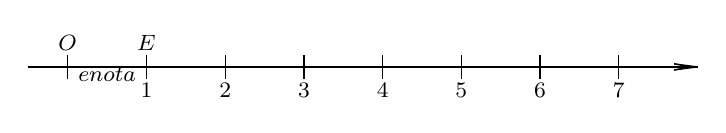
\begin{tikzpicture}
                        % \clip (0,0) rectangle (14.000000,10.000000);
                        {\footnotesize
                        
                        % Drawing segment a b
                        \draw [line width=0.016cm] (0.500000,0.500000) -- (9.000000,0.500000);%
                        
                        % Drawing arrow a b 1.00
                        \draw [line width=0.016cm] (8.702567,0.539158) -- (9.000000,0.500000);%
                        \draw [line width=0.016cm] (8.702567,0.539158) -- (8.900856,0.500000);%
                        \draw [line width=0.016cm] (8.702567,0.460842) -- (9.000000,0.500000);%
                        \draw [line width=0.016cm] (8.702567,0.460842) -- (8.900856,0.500000);%
                        
                        % Drawing segment c d
                        \draw [line width=0.016cm] (1.000000,0.350000) -- (1.000000,0.650000);%
                        
                        % Drawing segment e f
                        \draw [line width=0.016cm] (2.000000,0.350000) -- (2.000000,0.650000);%
                        
                        % Drawing segment g h
                        \draw [line width=0.016cm] (3.000000,0.350000) -- (3.000000,0.650000);%
                        
                        % Drawing segment i j
                        \draw [line width=0.016cm] (4.000000,0.350000) -- (4.000000,0.650000);%
                        
                        % Drawing segment k l
                        \draw [line width=0.016cm] (5.000000,0.350000) -- (5.000000,0.650000);%
                        
                        % Drawing segment m n
                        \draw [line width=0.016cm] (6.000000,0.350000) -- (6.000000,0.650000);%
                        
                        % Drawing segment o p
                        \draw [line width=0.016cm] (7.000000,0.350000) -- (7.000000,0.650000);%
                        
                        % Drawing segment r s
                        \draw [line width=0.016cm] (8.000000,0.350000) -- (8.000000,0.650000);%
                        
                        % Marking point O
                        \draw (1.000000,0.600000) node [anchor=south] { $O$ };%
                        
                        % Marking point E
                        \draw (2.000000,0.600000) node [anchor=south] { $E$ };%
                        
                        % Marking point 1
                        \draw (2.000000,0.400000) node [anchor=north] { $1$ };%
                        
                        % Marking point 2
                        \draw (3.000000,0.400000) node [anchor=north] { $2$ };%
                        
                        % Marking point 3
                        \draw (4.000000,0.400000) node [anchor=north] { $3$ };%
                        
                        % Marking point 4
                        \draw (5.000000,0.400000) node [anchor=north] { $4$ };%
                        
                        % Marking point 5
                        \draw (6.000000,0.400000) node [anchor=north] { $5$ };%
                        
                        % Marking point 6
                        \draw (7.000000,0.400000) node [anchor=north] { $6$ };%
                        
                        % Marking point 7
                        \draw (8.000000,0.400000) node [anchor=north] { $7$ };%
                        
                        % Marking point {enota}
                        \draw (1.500000,0.600000) node [anchor=north] { ${enota}$ };%
                        }
                    \end{tikzpicture}
                        
                \end{figure}

            \end{block}

            \begin{block}{}
                Vsako število zapišemo s \textbf{številko}. 
                Za zapis številke uporabljamo \textbf{števke}. Te so $0, 1, 2, 3, 4, 5, 6, 7, 8, 9$.
            \end{block}

            \begin{block}{}
                Posamezne števke večmestnega števila od desne proti levi predstavljajo: \textbf{enice}, \textbf{desetice}, \textbf{stotice}, \textbf{tisočice}, ...
            \end{block}

            \begin{block}{}
                Število, ki je zapisano s črkovnimi oznakami števk označimo s črto nad zapsiom črkovne oznake.
                $$ \overline{xy}=10x+y \quad \quad \quad \overline{xyz}=100x+10y+z$$
            \end{block}

            
        \end{frame}

        \begin{frame}
            \frametitle{Operacije v množici $\mathbb{N}$}

            \begin{alertblock}{Seštevanje}
                Poljubnima naravnima številoma $a$ in $b$ priredimo \textbf{vsoto} $\mathbf{\mathbf{a+b}}$.
            \end{alertblock}

            \begin{block}{}
                Število $a$ oziroma $b$ imenujemo \textbf{seštevanec}/\textbf{sumand}. 

                Število $a+b$ pa imenujemo \textbf{vsota}/\textbf{summa}. 
            \end{block}

            \begin{block}{}
                Vsota naravnih števil je naravno število: $a, b \in \mathbb{N} \Rightarrow a+b \in \mathbb{N}$.

            \end{block}

        \end{frame}

        \begin{frame}
            \begin{alertblock}{Množenje}
                Poljubnima naravnima številoma $a$ in $b$ priredimo \textbf{produkt} $\mathbf{\mathbf{a\cdot b}}$.
            \end{alertblock}

            \begin{block}{}
                Produkt naravnih števil je naravno število: $a, b \in \mathbb{N} \Rightarrow a\cdot b \in \mathbb{N}$.

            \end{block}

            \begin{block}{}
                Seštevanje in množenje sta \textit{dvočleni notranji operaciji}.
            \end{block}


        \end{frame}

        \begin{frame}
            \frametitle{Osnovni računski zakoni}

            Lastnosti:
            \begin{itemize}
                \item \textit{\textbf{komutativnost}} členov/zakon o zamenjavi členov: $a+b = b+a$.
                \item \textit{\textbf{asociativnost}} členov/zakon o združevanju členov: $(a+b)+c = a+(b+c)$.
            \end{itemize}

        \end{frame}

        \begin{frame}

            Lastnosti:
            \begin{itemize}
                \item \textit{\textbf{komutativnost}} faktorjev/zakon o zamenjavi faktorjev: $a \cdot b = b \cdot a$.
                \item \textit{\textbf{asociativnost}} faktorjev/zakon o združevanju faktorjev: $(a \cdot b) \cdot c = a \cdot (b \cdot c)$.
                \item \textit{\textbf{distributivnost}}/zakon o razčlenjevanju: $a \cdot (b+c) = a \cdot b + a \cdot c$.
                \item zakon o nevtralnem elementu: $a \cdot 1 = a$.
            \end{itemize}

        \end{frame}

        \begin{frame}
            \frametitle{Cela števila}

            \textbf{Množica celih števil}: 
                \begin{alertblock}{}
                    \centering\boldmath
                    $\mathbb{Z} = \{\ldots, -2, -1, 0, 1, 2, 3, \ldots\}$
                \end{alertblock}

                Množica celih števil je definirana kot unija treh množic:
                $$\mathbb{Z} = \mathbb{Z}^- \cup \{0\} \cup \mathbb{Z}^+$$

                \begin{itemize}
                    \item množica \textbf{pozitivnih celih števil} ($\mathbb{Z}^+$) -- naravna števila;
                    \item \textbf{število 0};
                    \item množica \textbf{negativnih celih števil} ($\mathbb{Z}^-$) -- nasprotna števila vseh naravnih števil.
                \end{itemize}
                
                \medskip
                \textbf{Nasprotno število} števila $a$ je $-a$.
        \end{frame}

        \begin{frame}

            Poleg seštevanja in množenja je kot notranja operacija množice celih števil
            definirano še \textbf{odštevanje}.

            \bigskip
            \textbf{\large{Odštevanje}}
            
            \bigskip
            Poljubnima naravnima številoma $a$ in $b$ priredimo \textbf{razliko} $\mathbf{a - b}$.
            
            \bigskip
            Odštevanje definiramo kot prištevanje nasprotne vrednosti: $a-b = a+(-b)$

            \bigskip
            Za odštevanje velja zakon \textit{\textbf{distributivnosti}}: $a \cdot (b-c) = a \cdot b - a
            \cdot c$.

        \end{frame}

        \begin{frame}
            \textbf{\large{Računski zakoni}}

            \smallskip
            \begin{itemize}
                \item Komutativnostni zakon: $$a+b = b+a ~\text{in}~ a \cdot b = b \cdot a$$
                \item Asociativnostni zakon: $$a+(b+c) = (a+b)+c ~\text{in}~ a \cdot (b \cdot c) = (a \cdot b) \cdot c$$
                \item Zakon o nevtralnem elementu: $$a+0 = a ~\text{in}~ a \cdot 1 = a$$
                \item Zakon o inverznem/nasprotnem elementu: $$a+(-a) = 0$$
                \item Distributivnostni zakon: $$a \cdot (b \pm c) = a \cdot b \pm a \cdot c$$
            \end{itemize}


        \end{frame}

        \begin{frame}
            \textbf{\large{Pravila za računanje s celimi števili}}

            \bigskip
            \begin{itemize}
                \item $-(-a)=a$
                \item $0\cdot a=0$
                \item $-1 \cdot a =-a$
                \item $(-a)+(-b)=-(a+b)$
                \item $(-a)\cdot b=-(a\cdot b)=a\cdot (-b)$
                \item $(-a)\cdot(-b)=a\cdot b$
            \end{itemize}
        \end{frame}

        \begin{frame}

        \end{frame}


    \subsection{Računanje z naravnimi in celimi števili}

        \begin{frame}
            \frametitle{Računanje z naravnimi in celimi števili}
        \end{frame}

    \subsection{Izraz, enačba, neenačba}

        \begin{frame}
            \frametitle{Izraz, enačba, neenačba}
        \end{frame}

        % \begin{frame}
        %     \frametitle{Neenačba}

        %     \begin{alertblock}{Neenačba}
        %         Neenačba je zapis, v katerem sta dva izraza v ustrezni relaciji.

        %             $$\left\langle \textmd{izraz_1}\right\rangle < \left\langle \textmd{izraz_2}\right\rangle $$
        %             $$\left\langle \textmd{izraz_1}\right\rangle \leq \left\langle \textmd{izraz_2}\right\rangle $$ 
        %             $$\left\langle \textmd{izraz_1}\right\rangle > \left\langle \textmd{izraz_2}\right\rangle $$ 
        %             $$\left\langle \textmd{izraz_1}\right\rangle \geq \left\langle \textmd{izraz_2}\right\rangle $$  

        %     \end{alertblock}
        % \end{frame}

    \subsection{Računanje s potencami z naravnimi eksponenti}

        \begin{frame}
            \frametitle{Računanje s potencami z naravnimi eksponenti}

            Potenca $\mathbf{a^n}$, pri čemer je $n \in \mathbb{N}$, je produkt $n$ faktorjev enakih $a$.

            \begin{figure}
                \includegraphics[scale=0.5]{Slike in skice/Potenca.jpg}
            \end{figure}
    
            \textbf{Pravila za računanje s potencami}:
            \begin{itemize}
                \item $\mathbf{a^n \cdot b^n = (ab)^n}$ - potenci z enakima eksponentoma zmnožimo tako, da zmnožimo osnovi in prepišemo eksponent
                \item $\mathbf{a^m \cdot a^n = a^{m+n}}$ - potenci z enako osnovo zmnožimo tako, da osnovo prepišemo in seštejemo eksponenta
                \item $\mathbf{(a^n)^m = a^{nm}}$ - potenco potenciramo tako, da osnovo prepišemo in zmnožimo eksponenta
            \end{itemize}

        \end{frame}

    \subsection{Razčlenjevanje izrazov}

        \begin{frame}
            \frametitle{Razčlenjevanje izrazov}
        \end{frame}

    \subsection{Razstavljanje izrazov v množici $\mathbb{Z}$}

        \begin{frame}
            \frametitle{Razstavljanje izrazov v množici $\mathbb{Z}$}
        \end{frame}

    \subsection{Reševanje linearnih in razcepnih enačb v množici $\mathbb{Z}$}

        \begin{frame}
            \frametitle{Reševanje linearnih in razcepnih enačb v množici $\mathbb{Z}$}
        \end{frame}

    \subsection{Reševanje linearnih neenačb v množici $\mathbb{Z}$}

        \begin{frame}
            \frametitle{Reševanje linearnih neenačb v množici $\mathbb{Z}$}
        \end{frame}

\include{Deljivost_izjave_množice}

\section{Racionalna števila}

\begin{frame}
    \sectionpage
\end{frame}

\begin{frame}
    \tableofcontents[currentsection, hideothersubsections]
\end{frame}

    \subsection{Številski ulomki}

        \begin{frame}
            \frametitle{Številski ulomki}
        \end{frame}

    \subsection{Racionalna števila}

        \begin{frame}
            \frametitle{Racionalna števila}
        \end{frame}

    \subsection{Algebrski ulomki}

        \begin{frame}
            \frametitle{Algebrski ulomki}
        \end{frame}

    \subsection{Računanje z ulomki}

        \begin{frame}
            \frametitle{Računanje z ulomki}
        \end{frame}

    \subsection{Potence s celimi eksponenti}

        \begin{frame}
            \frametitle{Potence s celimi eksponenti}
        \end{frame}

    \subsection{Pravila za računanje s potencami s celimi eksponenti}

        \begin{frame}
            \frametitle{Pravila za računanje s celimi eksponenti}
        \end{frame}

    \subsection{Premo in obratno sorazmerje}

        \begin{frame}
            \frametitle{Premo in obratno sorazmerje}
        \end{frame}

    \subsection{Odstotki}

        \begin{frame}
            \frametitle{Odstotki}
        \end{frame}


\section{Realna števila, statistika}

\begin{frame}
    \sectionpage
\end{frame}

\begin{frame}
    \tableofcontents[currentsection, hideothersubsections]
\end{frame}

    \subsection{Realna števila}

        \begin{frame}
            \frametitle{Realna števila}
        \end{frame}

    \subsection{Kvadratni in kubični koren}

        \begin{frame}
            \frametitle{Kvadratni in kubični koren}
        \end{frame}

        \begin{frame}
            \begin{exampleblock}{Naloga 563}
                Izračunaj in rezultat delno koreni.
                \begin{description}
                    \item<2->[(b)] $\displaystyle 4\sqrt{8}-\left(2\sqrt{5}+3\sqrt{8}\right)\sqrt{10}$
                    \item<3->[(č)] $\displaystyle\left(5\sqrt{3}+2\sqrt{27}\right)\left(\sqrt{5}-4\sqrt{12}+\sqrt{147}\right)$
                    \item<4->[(g)] $\displaystyle 8\sqrt{3}\left(\sqrt{2}-1\right)-\left(\sqrt{5}+2\sqrt{6}\right)\left(4-2\sqrt{2}\right)$  
                    \item<5->[(j)] $\displaystyle\left(2-4\sqrt{3}\right)\cdot 3\sqrt{2}-\left(2\sqrt{2}-3\sqrt{3}\right)^2$
                    \item<6->[(l)] $\displaystyle\left(3-2\sqrt{2}\right)^3-\left(\sqrt{8}-5\sqrt{2}\right)\left(-3\sqrt{2}\right)$
                    \item<7->[(o)] $\displaystyle\sqrt{300}-\sqrt{5-2\sqrt{6}}\cdot\sqrt{5+2\sqrt{6}}+\sqrt{5^4}$
                    \item<8->[(r)] $\displaystyle\sqrt{5\sqrt{3}-\sqrt{5}}\cdot\sqrt{2\sqrt{3}+2}-\left(\sqrt{5}\right)^3$  
                    \item<9->[(u)] $\displaystyle\left(\sqrt{17}-3\right)\sqrt{26+6\sqrt{17}}-\sqrt{2}\left(\sqrt{2}+\sqrt{6}\right)$
                \end{description}
            \end{exampleblock}
        \end{frame}

    \subsection{Intervali}

        \begin{frame}
            \frametitle{Intervali}
        \end{frame}

    \subsection{Absolutna vrednost}

        \begin{frame}
            \frametitle{Absolutna vrednost}
        \end{frame}

    \subsection{Sistem linearnih enačb}

        \begin{frame}
            \frametitle{Sistem linearnih enačb}
        \end{frame}

    \subsection{Obravnavanje linearnih enačb, neenačb, sistemov}

        \begin{frame}
            \frametitle{Obravnavanje linearnih enačb, neenačb, sistemov}
        \end{frame}

    \subsection{Absolutna in relativna napaka}

        \begin{frame}
            \frametitle{Absolutna in relativna napaka}
        \end{frame}

    \subsection{Sredine}

        \begin{frame}
            \frametitle{Sredine}
        \end{frame}

    \subsection{Razpršenost podatkov}

        \begin{frame}
            \frametitle{Razpršenost podatkov}
        \end{frame}

    \subsection{Prikazi}
        
        \begin{frame}
            \frametitle{Prikazi}
        \end{frame}

\section{Pravokotni koordinatni sistem, linearna funkcija}

\begin{frame}
    \sectionpage
\end{frame}

\begin{frame}
    \tableofcontents[currentsection, hideothersubsections]
\end{frame}

    \subsection{Pravokotni koordinatni sistem}

        \begin{frame}
            \frametitle{Pravokotni koordinatni sistem}
        \end{frame}

    \subsection{Razdalja med točkama in razpolovišče daljice}

        \begin{frame}
            \frametitle{Razdalja med točkama in razpolovišče daljice}
        \end{frame}

    \subsection{Ploščina trikotnika}

        \begin{frame}
            \frametitle{Ploščina trikotnika}
        \end{frame}

    \subsection{Osnovno o funkcijah}

        \begin{frame}
            \frametitle{Osnovno o funkcijah}
        \end{frame}

    \subsection{Linearna funkcija in premica}

        \begin{frame}
            \frametitle{Linearna funkcija in premica}
        \end{frame}

    \subsection{Oblike enačbe premice}

        \begin{frame}
            \frametitle{Oblike enačbe premice}
        \end{frame}

    \subsection{Presešišče premic}

        \begin{frame}
            \frametitle{Presešišče premic}
        \end{frame}

    \subsection{Sistem linearnih neenačb}

        \begin{frame}
            \frametitle{Sistem linearnih neenačb}
        \end{frame}

    \subsection{Modeliranje z linearno funkcijo}

        \begin{frame}
            \frametitle{Modeliranje z linearno funkcijo}
        \end{frame}

    \subsection{(i) Linearno programiranje}
        
        \begin{frame}
            \frametitle{(i) Linearno programiranje}
        \end{frame}



\end{document}